% !Mode:: "TeX:UTF-8"
%此为章节二模板
%\chapter、\section、\subsection、\subsubsection分别对应一二三四级标题
\chapter{相关理论与技术介绍}\label{ch:2}
\section{姿态估计}

物体姿态估计是机器人感知中的一个关键组成部分,它使得机器人能够在非结构化环境中进行精确的操作、导航和与物体的交互。在精确授粉的机器臂应用中,准确的姿态估计对于识别花朵的位置和朝向至关重要,从而确保授粉过程的精准与高效。机械臂执行精准的手眼协调能力依赖于其估计物体姿态并适应动态环境条件的能力。为提高姿态估计的精度,可采用多种传感方式,包括基于视觉、基于深度的传感技术以及传感器融合技术。本节将概述物体姿态估计的理论基础和关键技术。

\subsection{物体姿态估计的理论基础}




物体位姿估计涉及确定物体在给定坐标系中的位置和姿态。从数学角度看,位姿估计结合了平移和旋转,可以通过不同的方法表示。
 
 \subsubsection*{(1)齐次变换矩阵}
 \FloatBarrier
 \begin{figure}[htb]
 	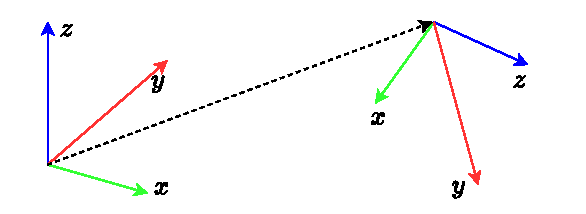
\includegraphics[width=0.7 \textwidth]{Homogeneous Transformation Matrix}
 	\caption[齐次变换矩阵]{齐次变换矩阵} % 中括号中内容为插图索引中显示内容,可在题注内容过长时使用
 	\label{fig:Homogeneous Transformation Matrix}
 \end{figure}
 
齐次变换矩阵是机器人学中广泛应用的一种表示方式,它将一个$3\times3$的旋转矩阵$R$和一个$3\times1$的平移向量$P$结合成一个$4\times4$变换矩阵$T$,如下所示:
\begin{equation}
	\label{equ:Homogeneous Transformation Matrix}
	T=
	\begin{bmatrix}
		R & P \\
		0 & 1 \\
	\end{bmatrix}=
	\begin{bmatrix}
		r_{11} & r_{12} & r_{13} & p_{1} \\
		r_{21} & r_{22} & r_{23} & p_{2} \\
		r_{31} & r_{32} & r_{33} & p_{3} \\
		0 & 0 & 0 & 1 \\
	\end{bmatrix}
\end{equation}
这种表示方法可以在统一框架中高效地组合和处理位姿,如\cref{fig:Homogeneous Transformation Matrix}所示。

 \subsubsection*{(2)欧拉角和四元数}
 
 \begin{figure}[htb]
 	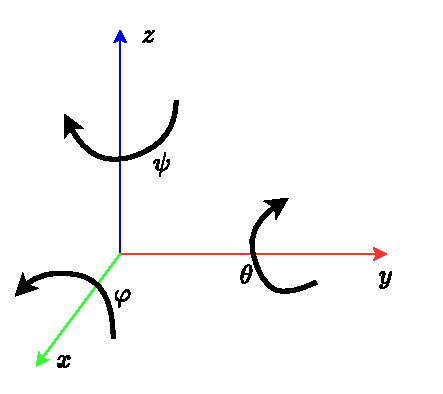
\includegraphics[width=0.43 \textwidth]{olErger.drawio}
 	\caption[欧拉角]{欧拉角} % 中括号中内容为插图索引中显示内容,可在题注内容过长时使用
 	\label{fig: olErger.drawio}
 \end{figure}
 
另一种表示姿态的方法是欧拉角,它引入了三个角度$(\phi,\theta,\psi)$,通过绕主要坐标轴的三次连续旋转来定义物体的朝向,如\cref{fig: olErger.drawio}所示,旋转矩阵$M$可以表示为三个旋转矩阵的乘积:
\begin{equation}
	\label{equ:oulEqu_1}
	M =R_{yz}(\phi)R_{zx}(\theta)R_{xy}(\psi) \\
\end{equation}
\begin{equation}
	\label{equ:oulEqu_2}
	M =
	\begin{bmatrix}
		1 & 0& 0  \\
		0 & \cos\phi & -\sin\phi \\
		0 & \sin\phi & \cos\phi  \\
	\end{bmatrix}
	\begin{bmatrix}
		\cos\theta & 0& \sin\theta  \\
		0 & 1 & 0 \\
		-\sin\theta & 0 & \cos\theta  \\
	\end{bmatrix}
	\begin{bmatrix}
		\cos\psi & -\sin\psi& 0  \\
		\sin\psi & \cos\psi & 0 \\
		0 & 0 & 1  \\
	\end{bmatrix}
\end{equation}

尽管欧拉角具有直观的优势,但它存在万向节锁死问题,即在某些情况下失去一个自由度,导致奇异性,因此不适用于连续运动应用。为了解决这一问题,四元数提供了一种更加稳定且简洁的表示方式,使用四个参数描述旋转,不会发生奇异性。它由一个标量和一个三维向量组成,表示如下:
\begin{equation}
	\label{equ:Quaternion}
	q=(w,x,y,z)
\end{equation}

$w$是标量部分,表示旋转的余弦分量,$(x,y,z)$是向量部分,表示旋转轴的正弦分量。四元数在实时应用中尤其具有优势,因为它们具有较高的计算效率和数值稳定性。

 \subsubsection*{(3)旋转向量}
 
  \begin{figure}[htbp]
 	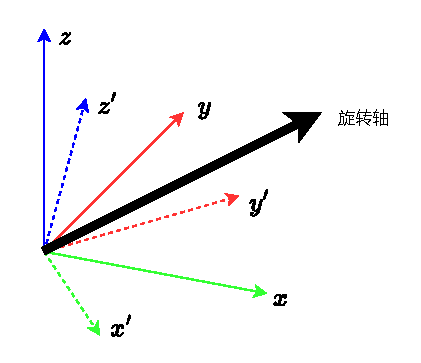
\includegraphics[width=0.43 \textwidth]{rotationVector.drawio}
 	\caption[旋转向量]{旋转向量} % 中括号中内容为插图索引中显示内容,可在题注内容过长时使用
 	\label{fig: rotationVector.drawio}
 \end{figure}
还有一种较为简洁的表示方式是旋转向量(轴-角表示),旋转向量$r$由旋转轴$v$和旋转角度$\theta$组成,定义如下:
\begin{equation}
	\label{equ:rotationVector}
	r=\theta v=(\theta v_{x},\theta v_{y},\theta v_{z})
\end{equation}

其中$v=(v_{x},v_{y},v_{z})$是旋转轴,它是一个单位向量,$\theta$ 是绕该轴旋转的角度,$r$ 是旋转向量,其方向是旋转轴,长度是旋转角度。这种表示方式通常用于优化问题中,当需要简洁但富有表达力的旋转描述时非常有用,如\cref{fig: rotationVector.drawio}所示,原坐标系$O_{xyz}$绕旋转轴旋转变换成坐标系$O_{x^{\prime}y^{\prime}z^{\prime}}$。


\subsection{坐标系与变换}
 \begin{figure}[htb]
	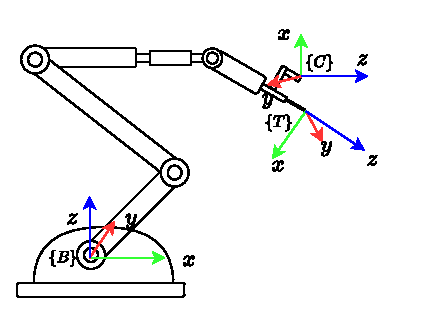
\includegraphics[width=0.6 \textwidth]{translation.drawio}
	\caption[机械臂中各个坐标系]{机械臂中各个坐标系} % 中括号中内容为插图索引中显示内容,可在题注内容过长时使用
	\label{fig:translation.drawio}
\end{figure}

在机器人视觉系统中,多个坐标系的精确变换至关重要,包括机器人基座坐标系(Base, \{B\})、末端TCP坐标系(Tool Center Point, TCP, \{T\})、相机坐标系(Camera, \{C\}),以及世界坐标系(World, \{W\}),如\cref{fig:translation.drawio}所示。这些坐标系之间的相互转换是保证机器人精准感知环境、执行任务的关键因素。特别是在动态任务中,坐标精度的误差可能直接影响机器人操作的成功率。因此,采用合理的运动学建模和手眼标定技术,建立精确的坐标转换关系,对于提升机器人系统的操作精度和稳定性具有重要意义。

\subsubsection*{(1)机械臂基座坐标系 }
机器人基座坐标系 \{B\} 作为整个机械臂系统的全局参考系,其原点通常位于机械臂的底座中心,$Z$轴垂直向上,$X$轴沿机械臂初始运动方向。所有关节和末端执行器的位置均相对于该坐标系进行定义。
\subsubsection*{(2)末端TCP 坐标系  }
TCP 坐标系\{T\} 由末端执行器(如夹爪)的工作点决定,通常不与机械臂法兰坐标系重合,而是存在一定的偏移量。其位置和姿态由机器人运动学方程(基于 Denavit-Hartenberg, DH 参数法)计算得出,即:
\begin{equation}
	\label{equ:coordinate_b_t}
	T^{B}_{T}=T^{B}_{J} \cdot T^{J}_{T} 
\end{equation}

其中,$T^{B}_{T} $为基座到机械臂关节的变换矩阵,$JT^{J}_{T}$为机械臂末端的工具偏移矩阵。通过该变换,可以从基座坐标系计算出 TCP 的位姿。
\subsubsection*{(3)相机坐标系 }
相机坐标系\{C\}由安装在机械臂上的视觉传感器(如RGB-D相机)定义,其原点位于相机光心,Z 轴朝向相机视线方向,X 轴向右,Y 轴向下。为了使相机与末端执行器协同工作,必须进行手眼标定(Hand-Eye Calibration),以求得相机与 TCP 之间的空间变换矩阵$T^{T}_{C}$。

\subsubsection*{(4)世界坐标系 }
在许多视觉任务中,机器人需要将检测到的目标点从相机坐标系 $\{C\}$ 映射到世界坐标系 $\{W\}$,这通常通过外部标定方法(如 AprilTag 或棋盘标定)获得变换矩阵 $T^{W}_{C}$。最终,目标点的世界坐标可以通过以下公式计算:
\begin{equation}
	\label{equ:coordinate_w_c}
	P_{W}=T^{W}_{C} \cdot P_{C} 
\end{equation}

其中,$P_{C} $为相机坐标系中的目标点,$P_{W}$为世界坐标系中的目标点。

\subsubsection*{(5)机械臂多坐标系转换的数学描述 }
2. 机械臂多坐标系转换的数学描述
各坐标系之间的变换通常采用齐次变换矩阵(Homogeneous Transformation Matrix),其形式为:
\begin{equation}
	\label{equ:coordinate_base}
	T^{A}_{B} =
	\begin{bmatrix}
		R_{3 \times 3} & t_{3\times 1}  \\
		0_{1 \times 3} & 1\\
	\end{bmatrix}
\end{equation}


其中$R_{3 \times 3}$为3$\times$3旋转矩阵,描述坐标系的方向变换; $t_{3 \times 1}$为3$\times$1平移向量,描述坐标系的位移变换。综合考虑所有坐标系的变换关系,目标点在基座坐标系中的表示可通过如下公式计算:

\begin{equation}
	\label{equ:coordinate_base_2}
	P_{B} = T^{B}_{T} \cdot T^{T}_{C} \cdot P_{C}
\end{equation}

这表明,若相机检测到某目标点$P_{C}$,可通过末端的手眼标定矩阵$T^{T}_{C}$以及机械臂运动学矩阵$T^{B}_{T}$进行转换,从而得到该目标点在基座坐标系中的位置。


\subsection{物体姿态估计技术}
\subsubsection{基于特征的姿态估计}
基于特征的物体姿态估计方法专注于检测和匹配图像中的显著特征。这些特征作为地标,帮助识别和定位三维空间中的物体。这些经典方法通常用于2D到3D的姿态估计任务,其中通过图像关键点与3D模型点的特征匹配来计算物体在相机坐标系中的姿态。

 \subsubsection*{(1)尺度不变特征变换}
尺度不变特征变换(SIFT) 在三维物体位姿估计任务中,SIFT算法通常用于从单张或多张二维图像中提取稳定的特征点,然后通过匹配这些特征点来推测物体在三维空间中的位置和朝向。

首先,通过从不同视角下拍摄的二维图像中提取SIFT特征点,算法能够在图像中找到具有显著差异和鲁棒性的局部特征。对于每个关键点,SIFT算法会生成一个包含局部图像梯度信息的描述符,确保在光照、旋转、尺度变化等变换下依然能准确地匹配相同的特征点。然后,使用这些匹配的特征点,结合相机的内外参(如相机的焦距和位置),通过几何计算方法(例如PNP算法)来估计物体的位姿。

在实际应用中,SIFT常与其他算法如PNP(Perspective-n-Point)和RANSAC结合使用,以增强位姿估计的准确性和鲁棒性。PNP算法用于通过一组已知3D点与其对应的2D投影点来估计相机的位置和朝向,而RANSAC则用于在特征匹配过程中剔除错误匹配点,从而提升结果的稳定性和准确性。

SIFT在三维物体位姿估计中的一个典型应用是增强现实(AR)。在增强现实应用中,SIFT被用来实时追踪物体的位置和姿态,并将虚拟信息叠加到实际场景中。这要求对物体的三维模型有准确的先验信息,并通过特征匹配来持续调整位姿估计,以确保虚拟物体能够正确地与现实世界中的物体对齐。

此外,SIFT也被广泛应用于3D重建任务中。在多视角的图像中提取到的特征点可以用于通过三角测量计算三维点的空间位置,进而重建出三维物体或场景。该过程中的特征匹配是实现精确重建的关键步骤,而SIFT提供了在不同视角下稳定且独特的特征描述符,极大地提高了匹配的成功率。
 \subsubsection*{(2)加速稳健特征}
SURF(加速稳健特征,Speeded-Up Robust Features) 是一种用于图像特征检测与描述的算法,旨在提高SIFT算法的计算效率,同时保持其稳健性。SURF算法由Bay等人于2006年提出,并在多个计算机视觉任务中广泛应用,如图像匹配、目标识别、三维重建和图像拼接等。与SIFT类似,SURF能够有效地检测到尺度、旋转和光照变化下稳定的特征点,但通过改进计算方法,显著提高了速度。

SURF的核心改进之一是采用Hessian矩阵来进行尺度空间中的特征点检测。通过近似计算Hessian矩阵,Hessian矩阵的形式如下:
\begin{equation}
	\label{equ:Hessian}
	H(x,\sigma) =
	\begin{bmatrix}
		D_{xx}(x,\sigma) & D_{xy}(x,\sigma)  \\
		D_{xy}(x,\sigma)  & D_{yy}(x,\sigma) \\
	\end{bmatrix}
\end{equation}

其中$D_{xx}(x,\sigma)$ ,$D_{xy}(x,\sigma)$ ,$D_{yy}(x,\sigma)$ 是图像的二阶偏导数,表示图像在各方向的曲率。Hessian矩阵的特征值能够反映图像中局部区域的强度变化,从而识别出重要的特征点。

SURF能够在不同尺度下快速检测到图像中的显著特征点。此外,SURF通过引入积分图的加速技术,使得图像梯度的计算更加高效,从而降低了计算复杂度,相较于SIFT在处理速度上具有显著优势。

为了实现旋转不变性,SURF为每个特征点分配一个主方向,该方向基于关键点邻域内的梯度方向进行计算。SURF的特征描述符基于Haar小波响应,通过计算关键点邻域内的局部梯度来生成描述符。这些描述符能够高效地描述图像的局部结构,并且在光照、旋转和尺度变化下保持不变性。

SURF在计算效率上优于SIFT,是一个在许多计算机视觉任务中广泛应用的强大工具,尤其是在需要快速特征提取和匹配的场景中,如全景拼接、实时物体追踪和三维重建等。
 \subsubsection*{(3)Oriented FAST and Rotated BRIEF}
ORB(Oriented FAST and Rotated BRIEF)是一种结合了FAST角点检测和BRIEF描述符的特征点检测与描述算法,主要用于计算机视觉中的特征匹配和图像配准。它由Ethan Rublee等人于2011年提出,旨在提高传统方法在旋转不变性和计算效率上的性能。ORB不仅具备较高的鲁棒性,还能在实时应用中保持较快的运行速度,因此被广泛应用于诸如物体识别、图像拼接和机器人定位等领域。

ORB的核心思想是首先使用FAST(Features from Accelerated Segment Test)角点检测器来检测图像中的角点。FAST是一个高效的角点检测方法,通过分析像素点周围区域的亮度变化来确定角点的存在。与传统的Harris角点检测器相比,FAST具有更快的计算速度,适合于实时处理。但仅使用FAST检测到的角点并不足以解决旋转和尺度变化的问题,因此ORB引入了对角点的方向性分析,以实现对旋转变化的鲁棒性。

为了进一步提高描述符的质量和匹配的准确性,ORB采用了BRIEF(Binary Robust Independent Elementary Features)描述符。BRIEF通过比较特征点邻域内像素对的亮度值来生成二进制字符串,用以描述特征点周围的局部图像信息。这使得描述符具有非常高的计算效率,并且容易存储。然而,BRIEF本身对旋转不具备鲁棒性,因此ORB在生成BRIEF描述符之前,会先为每个角点计算一个主方向,使得生成的描述符在旋转后的图像中仍能保持一致。

尽管ORB并不像SIFT或SURF那样直接支持尺度不变性,但通过图像金字塔结构,ORB可以在不同尺度下检测和描述特征点,从而实现一定程度的尺度不变性。这使得ORB在处理图像中的尺度变化时仍然能够保持较好的表现。此外,ORB具有较强的抗噪声能力,能够在低质量或含有噪声的图像中进行有效的特征匹配和追踪。

\subsubsection{基于深度学习的方法}
与传统方法不同,基于深度学习的方法利用大规模数据集和卷积神经网络(CNN)直接从原始图像数据中估算物体姿态,从而省略了显式的特征提取。这些方法能够有效处理复杂场景,包括遮挡和视角变化,传统方法可能无法应对这些情况。以下是一些在物体姿态估计中突出的深度学习方法:
 \subsubsection*{(1)PoseNet}
 \begin{figure}[htb]
 	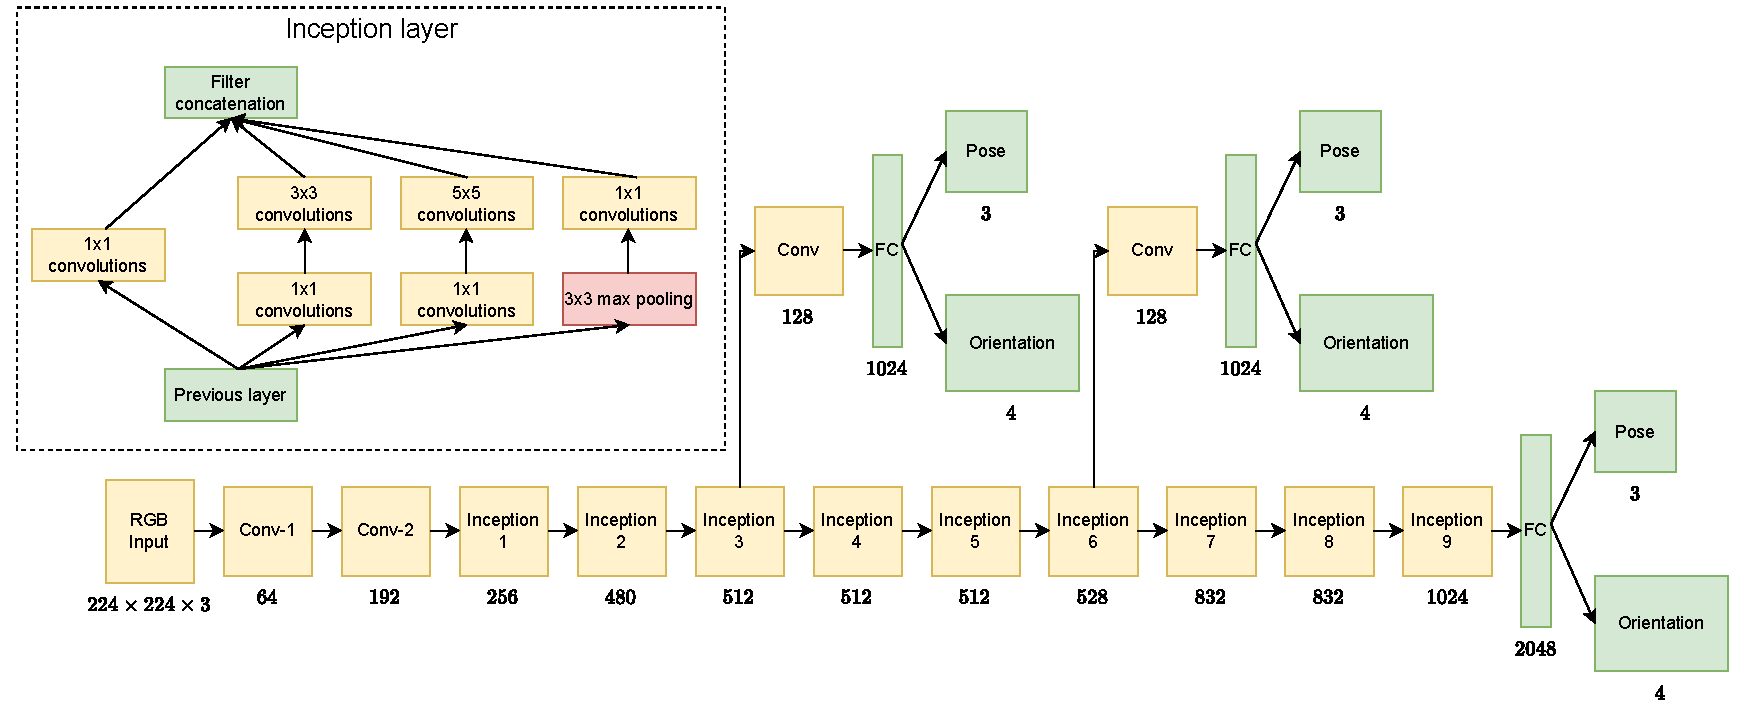
\includegraphics[width=1 \textwidth]{posenet.drawio}
 	\caption[PoseNet模型结构]{PoseNet模型结构} % 中括号中内容为插图索引中显示内容,可在题注内容过长时使用
 	\label{fig:posenet.drawio}
 \end{figure}
 
PoseNet是一种基于深度学习的方法,通过卷积神经网络(CNNs)直接从单个RGB图像预测6自由度(6-DoF)的相机位姿。这种方法无需显式特征匹配,提高了对环境变化的鲁棒性,并能推广到不同的场景。与依赖人工特征提取的方法不同,PoseNet通过监督学习直接从图像像素学习到相机位姿的映射关系。
PoseNet的核心方法涉及训练一个CNN,通常基于GoogleNet或ResNet等架构,以预测相机位姿。该网络由卷积层组成,用于特征提取,随后是全连接层,用于回归相机的6D位姿向量。该向量包括三个空间坐标和四元数表示的方向,从而可以从单张图像中实现稳健的位姿估计。如\cref{fig:posenet.drawio}所示。

在训练过程中,PoseNet用了一个同时平衡位置和方向误差的损失函数。损失函数定义如下:
\begin{equation}
	\label{equ:poseNet}
	L = || x - \hat{x} ||_{2} + \beta||q - \hat{q}||_{2}
\end{equation}

其中, $x$和$q$分别是真实位置和方向,而$\hat{x}$和$\hat{q}$是预测值。权重超参数$\beta$引入,以平衡平移误差和旋转误差的影响,从而确保稳定和准确的位姿预测。

这种方法使PoseNet即使在传统方法因遮挡或缺乏显著特征而失效的情况下仍能有效工作。通过利用CNN,PoseNet能够从图像中提取稳健的特征表示,从而在复杂环境中实现可靠的位姿估计。

 \subsubsection*{(2)DenseFusion}
  \begin{figure}[htb]
 	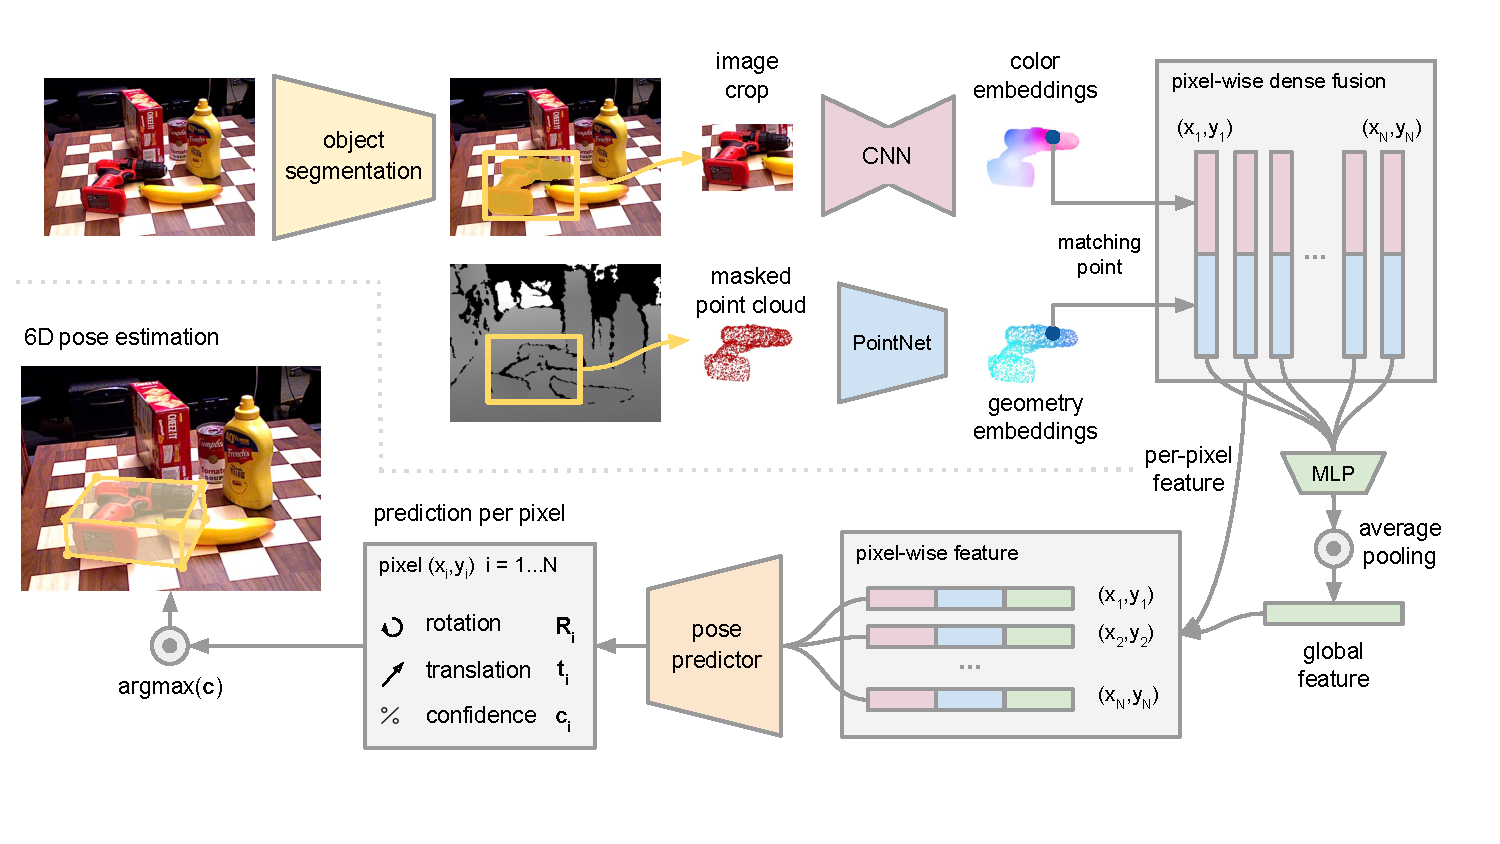
\includegraphics[width=1 \textwidth]{denseFusionoverall_workflow}
 	\caption[DenseFusion工作流程图]{DenseFusion工作流程图} % 中括号中内容为插图索引中显示内容,可在题注内容过长时使用
 	\label{fig:denseFusionoverall_workflow}
 \end{figure}
 
DenseFusion 是一种基于深度学习的 6D 物体位姿估计框架,利用 RGB 和深度(RGB-D)数据 实现精准而鲁棒的位姿预测。不同于依赖手工特征的传统方法,DenseFusion 采用 像素级特征融合,分别提取 RGB 和深度特征,然后在每个像素级别进行融合,形成密集的特征表示。这种方法能够同时捕获外观信息和几何信息,使得网络在 遮挡和复杂环境 下依然能够保持较高的估计精度。

DenseFusion 的网络由 特征提取、位姿估计和位姿优化 三个关键阶段组成。首先,CNN 主干网络(如 ResNet) 提取 RGB 特征,而 基于 PointNet 的网络 处理来自 3D 点云的 深度信息。这些特征随后在像素级别进行融合,确保每个像素都携带丰富的视觉和空间数据。融合后的特征通过 多层感知机(MLP) 进行处理,直接预测物体的 6D 位姿(旋转 + 平移)。然而,由于初始预测可能存在误差,DenseFusion 还包含一个 位姿优化模块,该模块通过最小化预测位姿与观测深度数据之间的差异,迭代优化位姿估计,显著提高最终的估计精度,工作流程如\cref{fig:denseFusionoverall_workflow}所示。

DenseFusion 的损失函数用来最小化3D模型上的采样点在真实位姿下的坐标与在预测位姿下的坐标之间的欧氏距离的均值。并且针对非对称和对称物体选取了不同的损失函数,其中非对称物体的损失函数为:
\begin{equation}
	\label{equ:denseFusion_1}
	L^{p}_{i} = \frac{1}{M}\sum\limits_{j}||(Rx_{j} +t)-(\hat{R}_{i}x_{j} + \hat{t}_{i})||
\end{equation}

其中,$x_{j}$表示从物体三维模型中随机选取的M个三维点中的第 j 个点,$R$和$t$是真实姿态,$\hat{R}_{i}$和$\hat{t}_{i}$是根据第 i 个密集像素的融合嵌入生成的预测姿态。

对称物体的损失函数为:
\begin{equation}
	\label{equ:denseFusion_2}
	L^{p}_{i} = \frac{1}{M}\sum\limits_{j}\min\limits_{0<k<m}||(Rx_{j} +t)-(\hat{R}_{i}x_{j} + \hat{t}_{i})||
\end{equation}

对所有预测的每个高密度像素的姿态进行优化,就是最小化每个高密度像素损失的平均值,用密集像素置信度对每个密集像素的损失进行加权,并添加第二个置信度正则化项,最终的损失函数为:
\begin{equation}
	\label{equ:denseFusion_3}
	L= \frac{1}{N}\sum\limits_{i}(L_{i}^{p}c_{i} - w\log(c_{i}))
\end{equation}

其中,$N$为从片段的$P$个元素中随机采样的密集像素特征的数量,$w$为平衡超参数。
\subsubsection*{(3)PVNet}
  \begin{figure}[htb]
	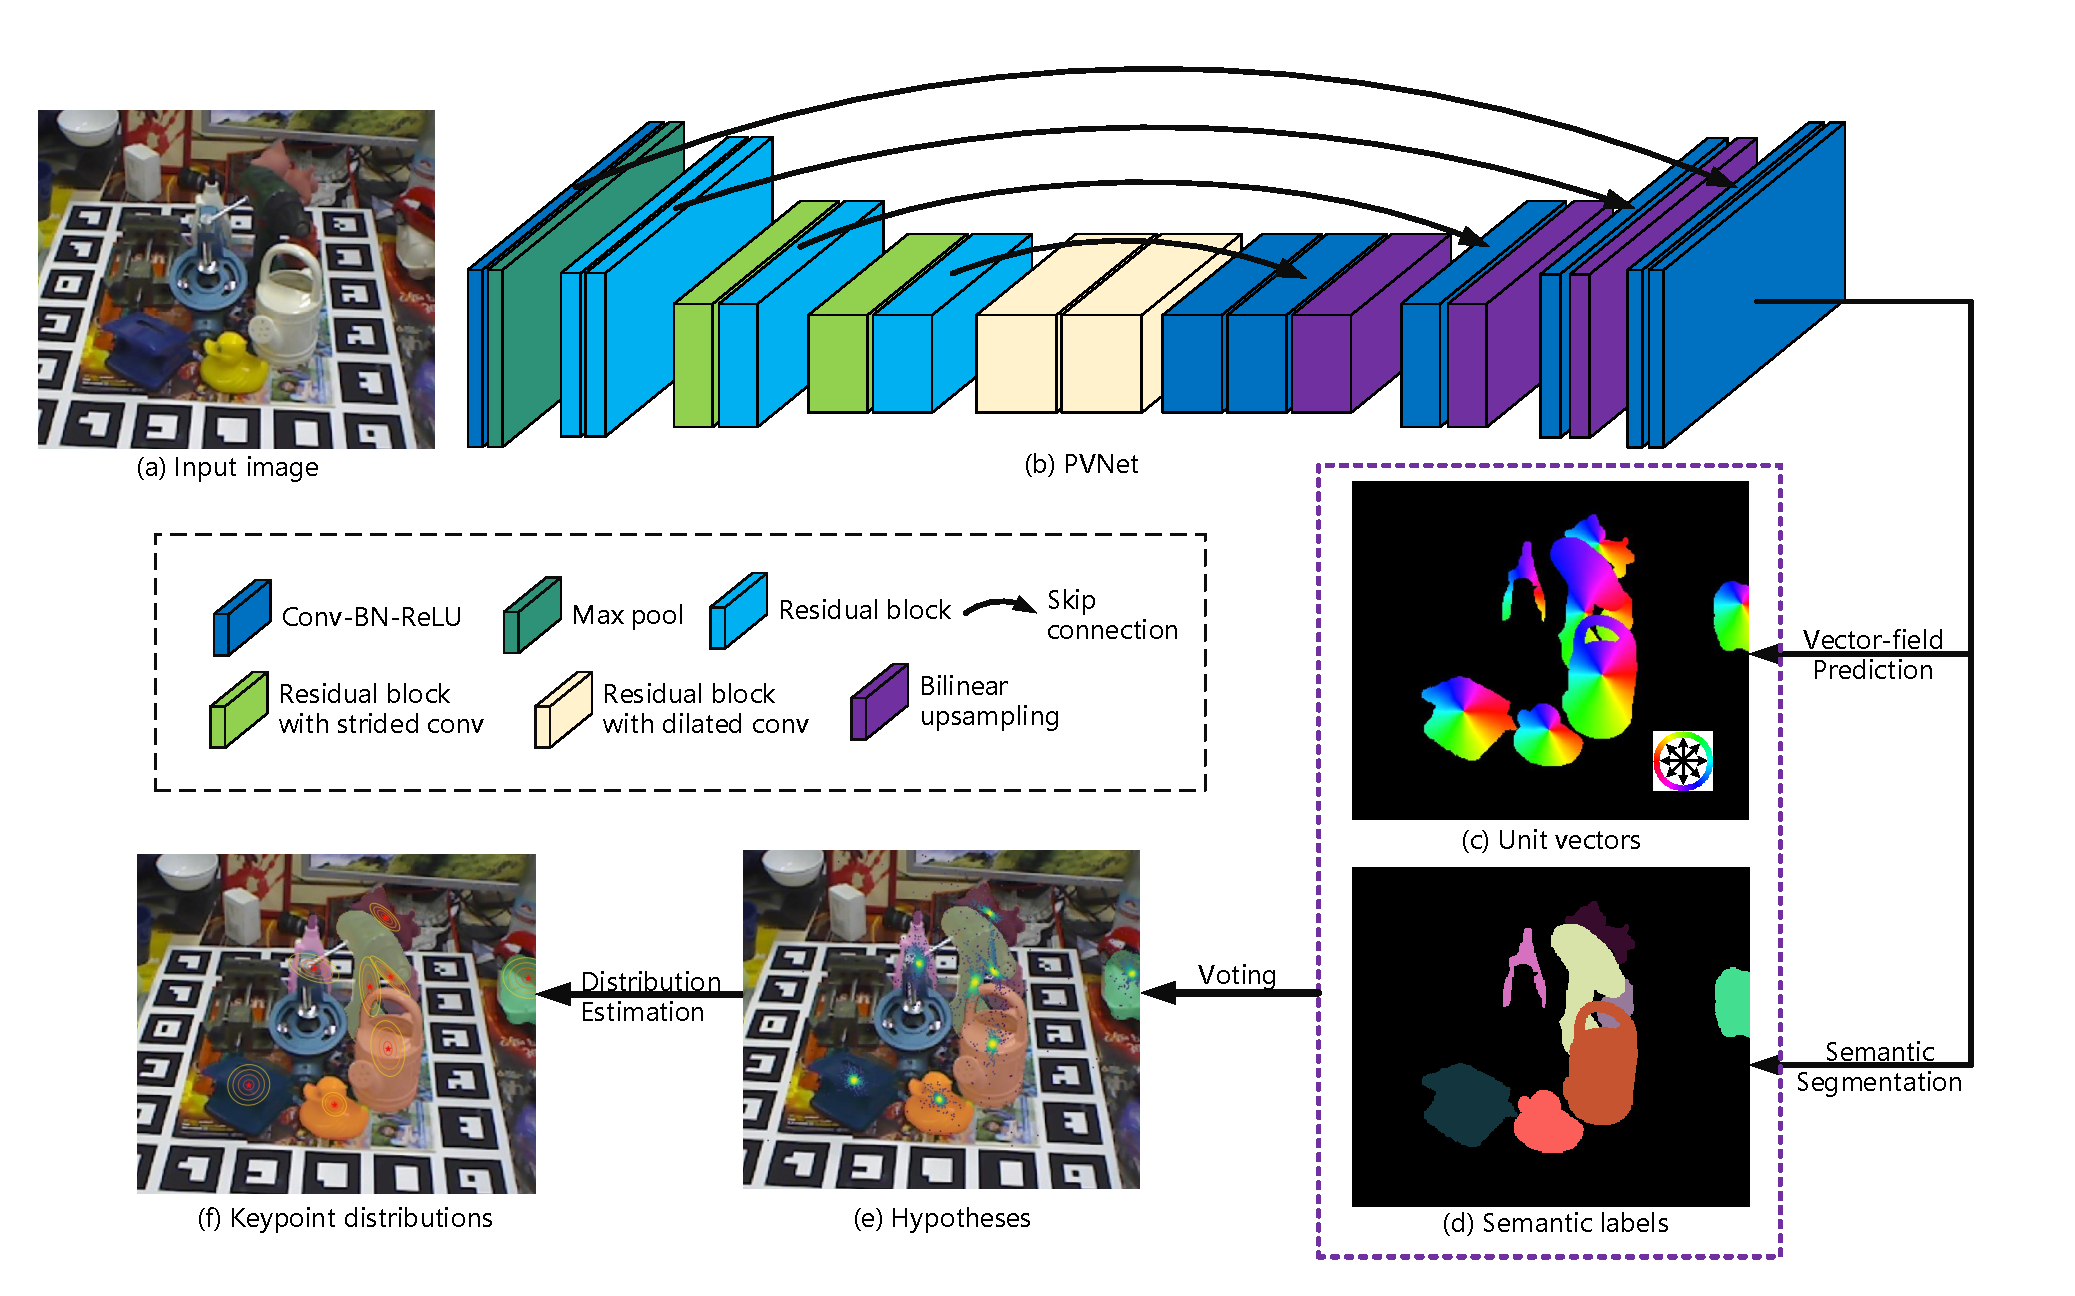
\includegraphics[width=1 \textwidth]{pvnet}
	\caption[关键点定位概述]{关键点定位概述: (a) Occlusion LINEMOD 数据集图像。(b) PVNet 的架构。(c)
		指向物体关键点的像素矢量。(d) 语义标签。(e) 通过投票产生的关键点位置假设。投票得分较高的
		投票得分越高的假设越亮。(f) 根据假设估算出的关键点位置的概率分布。分布的
		分布的平均值用红星表示,协方差矩阵用椭圆表示。} % 中括号中内容为插图索引中显示内容,可在题注内容过长时使用
	\label{fig:pvnet}
\end{figure}
PVNet(姿态与视角网络)是一种基于深度学习的6D物体姿态估计方法,旨在从单张RGB图像中估计物体的位置信息(平移)和方向信息(旋转)。与传统方法不同,PVNet能够有效应对视角变化和部分遮挡问题,这使得它在现实场景中表现尤为出色,尤其是当物体可能部分被遮挡或以非标准角度被观察时。它能够在这些具有挑战性的条件下准确估计物体的姿态,远优于早期在泛化能力方面表现较差的技术。

PVNet的核心使用卷积神经网络(CNN)从输入图像中提取高层次特征,然后预测物体上的关键点。这些关键点对于确定物体的姿态至关重要。通过将这些关键点与物体的3D模型进行匹配,网络能够计算出物体的6D姿态(平移和旋转)。此外,PVNet还能够估计物体的视角,从而进一步提高估计精度,能够有效应对不同的观察角度和姿态变化。\cref{fig:pvnet}展示了PVNet工作流程概述。

PVNet的一大优势是它对遮挡的鲁棒性。在许多现实应用中,物体往往会被部分遮挡,这使得传统的姿态估计方法难以应对。通过聚焦于物体的关键点,即使物体的一部分不可见,PVNet依然能够生成准确的姿态估计。这一特性使得它在机器人领域尤其有用,因为在机器人操作中,物体并不总是完全可见的。

PVNet是一个端到端的深度学习框架,这意味着它能够直接从原始图像中学习,无需手动进行特征工程。这简化了PVNet在各种应用中的部署,包括机器人、增强现实(AR)和自动驾驶汽车等领域。


\section{机械臂运动规划}
运动规划是机器人学中的一项关键任务,特别是对于介尺度机械臂,它们被设计用于执行精确和细致的运动。这些机器人臂广泛应用于需要高精度的领域,如精准授粉、外科机器人和微组装等。运动规划的目标是生成一条轨迹,使机器人臂能够从初始位置移动到目标位置,同时避开障碍物并优化运动效率。在环境要求机器人臂必须适应动态条件时,运动规划任务会变得更加复杂,使得适应性成为规划过程的关键因素。
传统的运动规划方法,如插值法,在结构化环境中有效,提供了平滑和高效的路径。然而,随着机器人任务的复杂性增加,特别是在非结构化环境中,新的技术如深度学习逐渐成为有价值的工具。这些方法使机器人臂能够通过从环境反馈和传感数据中学习,自主地调整到新的情境中。本文讨论了基于传统插值法的方法和现代深度学习方法,并强调了每种方法在解决机器人运动规划挑战,特别是精准授粉任务中的贡献。
在执行精密操作时,介尺度机械臂面临几项关键挑战。包括:
1.	精度与准确性:高精度对于执行如花粉传播等细致任务至关重要,因为即便是微小的运动偏差也可能导致失败。机器人臂必须执行高精度的运动,通常需要达到亚毫米级的精度,以避免损坏易碎的物体或组件。
2.	动态环境:机器人臂必须在动态环境中工作,障碍物或物体可能会不可预测地移动,这要求机器人臂实时调整其轨迹。在某些应用中,环境可能还包括变化的光照条件或杂乱的场景,进一步增加了运动规划的难度。
3.	有限的工作空间与障碍物:许多机器人臂在空间有限的环境中操作,必须高效地避免碰撞。路径规划必须考虑到障碍物以及与其他物体或机器人系统的潜在干扰,确保机器人臂在有限的工作空间内安全有效地移动。
当这些因素相互结合时,运动规划的复杂性增加,因此需要结合传统方法与深度学习技术,以达到最佳性能。



\subsection{传统运动规划方法}

在实际应用中,插值方法被广泛用于路径生成和轨迹规划。例如,在精准授粉中,机器人臂需要沿着预定义路径运动,同时避开障碍物并减少对脆弱花朵的影响。通过使用三次或五次样条插值,机器人臂可以生成最小化突然运动的轨迹,确保路径点之间的平稳过渡。
插值方法使机器人能够高效地跟随复杂路径,无论是在关节角度还是末端执行器的位置之间进行插值。在授粉任务中,机器人臂必须从一朵花移动到另一朵花,运动的平滑性至关重要,以避免对花朵造成损害。使用三次和五次样条插值确保机器人可以平稳地从一个位置到另一个位置,调整花朵的朝向等环境变化。
通过生成优化路径,机器人臂可以减少不必要的运动,从而提高任务效率。在精准授粉的背景下,减少运动时间对于提高产量和提升系统性能非常重要。
插值法长期以来一直是机器人臂运动规划的核心技术。它通过计算预定义路径点之间的中间点,生成机器人臂的平滑路径。几种插值方法在实践中被广泛应用:

\subsubsection{线性插值(Lerp)}
 \begin{figure}[htb]
	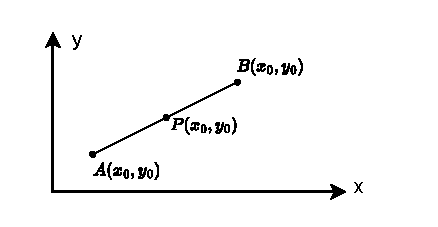
\includegraphics[width=0.5\textwidth]{lerp.drawio}
	\caption[线性插值]{线性插值} % 中括号中内容为插图索引中显示内容,可在题注内容过长时使用
	\label{fig:lerp.drawio}
\end{figure}
线性插值(Linear Interpolation,简称 Lerp)是一种在两个已知数据点之间计算中间值的方法。其基本思想是基于一个插值因子$t$(通常在 0 到 1 之间),按照比例在两个点之间进行平滑过渡,如\cref{fig:lerp.drawio}所示。线性插值广泛应用于计算机图形学、信号处理、运动规划、物理仿真、机器人路径控制等领域。
在机器人运动控制中,Lerp 可用于在已知的起始位置和目标位置之间生成平滑的运动轨迹,以确保运动的连续性和稳定性。

给定两个点$A$和$B$,其坐标分别为$A(x_{0},y_{0})$和$B(x_{1},y_{1})$,线性插值计算一个参数$t(t\in[0,1])$对应的插值点$P(x,y)$:
\begin{equation}
	\label{equ:Lerp:1}
	P=A + t(B-A)
\end{equation}

然而,对于需要平滑过渡的复杂任务,线性插值通常过于简单。例如,当机器人在两个点之间改变朝向时,运动不够平滑。
\subsubsection{球面线性插值(Slerp)} 
 \begin{figure}[htb]
	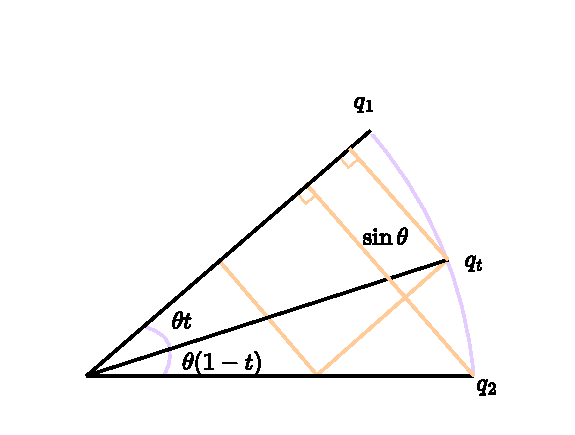
\includegraphics[width=0.6\textwidth]{Slerp.drawio}
	\caption[球面线性插值]{球面线性插值} % 中括号中内容为插图索引中显示内容,可在题注内容过长时使用
	\label{fig:Slerp.drawio}
\end{figure}
球面线性插值(Slerp)是一种用于单位向量或单位四元数之间的平滑插值方法,确保旋转沿着球面最短路径进行。它广泛应用于 3D 计算机图形学、机器人运动控制和动画平滑过渡等场景。Slerp 的核心原理是基于两个旋转状态的夹角,通过三角函数插值计算出中间旋转状态,使得旋转过程保持恒定角速度,从而避免线性插值(Lerp)可能产生的旋转变形问题,如\cref{fig:Slerp.drawio}所示。

Slerp 的计算公式如下:给定两个单位四元数$q_{1}$和$q_{2}$,以及插值因子$t(t\in[0,1])$,插值点$q(t)$可表示为:
\begin{equation}
	\label{equ:Slerp:1}
	Slerp(q_{1},q_{2},t)=\frac{\sin((1-t)\theta)}{\sin(\theta)}q_{1} + \frac{\sin(t\theta)}{\sin(\theta)}q_{2}
\end{equation}

其中,$\theta$是四元数$q_{1}$和$q_{2}$之间的夹角,由点积计算得到:
\begin{equation}
	\label{equ:Slerp:2}
	\cos(\theta)=q_{1} \cdot{q_{2}}
\end{equation}

Slerp 的主要优势在于,它可以沿球面最短路径插值,避免 Lerp 可能造成的旋转失真,并且保持恒定角速度,使得旋转过渡更加自然。
\subsubsection{三次样条插值}  
 \begin{figure}[htb]
	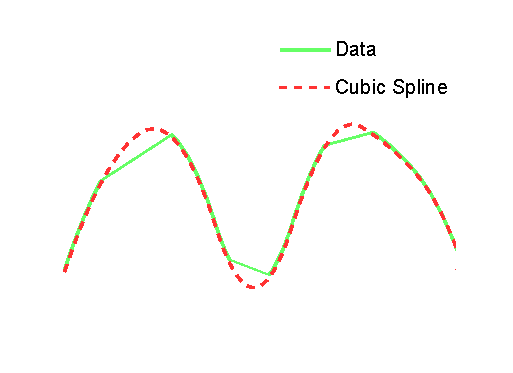
\includegraphics[width=0.5\textwidth]{Cubic Spline Interpolation.drawio}
	\caption[三次样条插值示意图]{三次样条插值示意图} % 中括号中内容为插图索引中显示内容,可在题注内容过长时使用
	\label{fig:Cubic Spline Interpolation.drawio}
\end{figure}
三次样条插值(Cubic Spline Interpolation)是一种用于平滑插值的方法,能够在数据点之间创建连续、光滑的曲线。与高阶多项式插值相比,三次样条插值能够有效避免振荡现象,因此广泛应用于计算机图形学、机器人路径规划、数据拟合和信号处理等领域。其基本思想是使用多个三次多项式函数,在相邻数据点之间进行插值,同时确保整体曲线的光滑性,如\cref{fig:Cubic Spline Interpolation.drawio}所示。

在三次样条插值中,对于一组数据点$(x_{0},y_{0}),(x_{1},y_{1}),(x_{2},y_{2}),...,(x_{n},y_{n})$,系统需要在每两个相邻点之间构造一个三次多项式$S_{i}(x)$来表示曲线段。该多项式的形式为:
\begin{equation}
	\label{equ:Cubic Spline Interpolation 1}
	S_{i}(x) = a_{i} + b_{i}(x-x_{i}) + c_{i}(x-x_{i})^{2} + d_{i}(x-x_{i})^{3}  
\end{equation}

为了确保整体曲线的平滑性,系数$a_{i},b_{i},c_{i},d_{i}$需要满足一系列约束条件。首先,插值曲线必须经过所有数据点,即满足插值条件。其次,在相邻的插值段之间,一阶导数必须连续,以确保曲线的平滑过渡。此外,二阶导数也必须连续,以保持曲率的平滑性。最后,还需要引入适当的边界条件,例如自然边界(两端二阶导数为零)、夹持边界(指定端点的一阶导数)或周期性边界(确保首尾曲线平滑衔接)。这些条件共同构成了一个三对角线性方程组,通过求解该方程组,即可得到每段插值函数的系数。

在具体计算过程中,我们首先计算数据点之间的间隔$h_{i} = x_{i+1} - x_{i}$,然后根据二阶导数的连续性条件构造方程组。解出二阶导数$M_{i}$之后,可以进一步计算各段插值多项式的系数:

\begin{equation}
	\label{equ:Cubic Spline Interpolation 2}
	\begin{split}
		b_{i} &= \frac{y_{i+1} - y_{i}}{h_{i}} - \frac{h_{i}}{6}(M_{i+1} + 2M_{i})   \\
		c_{i} &= \frac{M_{i}}{2} ,d_{i} = \frac{M_{i+1} - M_{i}}{6H_{i}}
	\end{split}
\end{equation}

三次样条插值在多个领域有广泛应用。例如,在机器人路径规划中,它可用于计算平滑的运动轨迹,确保机械臂运动过程中没有突兀的加速或减速变化,从而提高运动的稳定性。在计算机动画中,三次样条能够让角色的运动过渡更加自然,避免生硬的动作切换。此外,在数据拟合和图像处理领域,三次样条插值可用于创建高精度的光滑曲线,适用于信号平滑和图像变形处理。

与其他插值方法相比,三次样条插值的优势在于其高平滑性和稳定性。它能够有效避免拉格朗日插值或高阶多项式插值可能出现的振荡现象,同时提供更加可控的曲线形状。然而,由于需要解一个线性方程组,其计算量比线性插值或分段线性插值略大。


\subsection{深度学习方法}
尽管传统的插值方法在控制环境中有效,但深度学习在解决更复杂的动态运动规划挑战中越来越受到关注。深度学习技术在解决复杂运动规划问题,特别是在动态或非结构化环境中,越来越受到重视。深度学习使机器人臂能够从传感器数据中学习,从而提高其在实时环境中的适应性和决策能力。

\subsubsection{DQN}
 \begin{figure}[htb]
	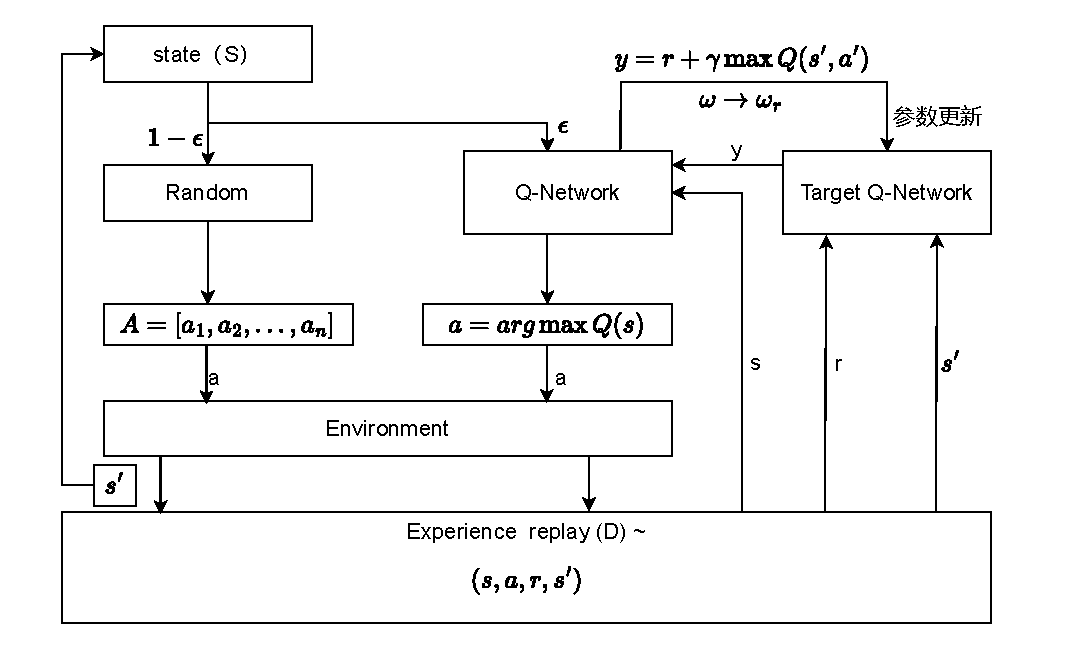
\includegraphics[width=0.85\textwidth]{dqn.drawio}
	\caption[DQN算法流程图]{DQN算法流程图} % 中括号中内容为插图索引中显示内容,可在题注内容过长时使用
	\label{fig:dqn.drawio}
\end{figure}
深度Q网络(Deep Q-Network, DQN)是一种结合深度学习与强化学习的方法,旨在解决高维状态空间下的离散动作决策问题。它最早由 DeepMind 提出。通过CNN处理环境输入,使Q-learning能够适用于复杂任务,如机器人控制、机械臂路径规划、避障和自主抓取等。DQN在Q-learning的基础上引入了深度神经网络,利用 CNN 提取图像特征,从而实现端到端的智能决策。

DQN的核心思想是使用一个深度神经网络$Q(s,a;\theta)$近似$Q$函数,并通过经验回放和目标网络提高训练稳定性。在 Q-learning中,Q值表示机器人在某一状态下执行某一动作的未来累积奖励。DQN通过贝尔曼方程进行Q值更新:
\begin{equation}
	\label{equ:DQN}
	Q(s,a) = r + \gamma\max Q(s^{\prime},a^{\prime})
\end{equation}

其中,$\gamma$是折扣因子,平衡短期与长期奖励。DQN采用CNN 处理高维输入(如图像或点云),再通过全连接层输出各个动作的Q值,最终根据 $\epsilon$-贪心策略选择最优动作,算法流程如\cref{fig:dqn.drawio}所示。

为了提高训练效率和稳定性,DQN 采用了三项关键改进。首先是经验回放(Experience Replay),它通过存储历史经验$(s,a,r,s^{\prime})$并随机采样进行训练,从而打破数据相关性,提高数据利用率。其次是目标网络(Target Network),该方法通过引入一个更新较慢的Q目标网络$Q(s,a,r,s^{\prime})$,防止训练过程中的目标值振荡。此外,DQN 还采用奖励裁剪(Reward Clipping) 来限制奖励范围,避免Q值爆炸。

\subsubsection{DDQN}
双重深度Q网络(Double Deep Q-Network, DDQN)是对 DQN 的改进版本,旨在解决 Q 值过高估计(Q-value Overestimation)的问题,提高强化学习的稳定性和策略优化能力。在 DQN 中,机器人使用Q-learning 进行决策,Q值表示在特定状态下执行某个动作的累积奖励。然而,由于DQN使用同一个网络进行动作选择和Q值评估,容易导致某些动作的Q值被过高估计,进而影响策略收敛。为了解决这一问题,DDQN 通过分离动作选择和Q值计算,降低Q值过高估计的影响,使得机器人在训练过程中更加稳定,并能更精准地选择最优策略。
在 DDQN中,Q值的计算方式进行了关键改进。与DQN直接使用目标网络计算最大Q值不同,DDQN采用两个Q网络:一个是在线Q网络(Online Network),用于选择下一个状态的最优动作;另一个是目标Q网络(Target Network),用于评估这个动作的Q值。在 DDQN中,机器人首先使用在线网络选择最优动作$a^{*}$:
\begin{equation}
	\label{equ:DDQN1}
	a^{*} = arg\max Q_{online}(s^{\prime},a^{*})
\end{equation}
然后使用目标网络评估该动作的Q值:
\begin{equation}
	\label{equ:DDQN2}
	yDDQN = r + \gamma Q_{target}(s^{\prime},a^{*})
\end{equation}
这种方式确保了动作选择和Q值评估分别由不同的网络完成,避免了Q值的过高估计问题,提高了强化学习的可靠性和泛化能力。

在训练过程中,DDQN采用与DQN相似的流程。首先,机器人与环境交互,执行动作并存储经验数据$(s,a,r,s^{\prime})$到经验回放池(Replay Buffer)。然后,从经验池中随机采样数据,计算DDQN的目标Q值,并使用梯度下降更新在线网络的参数。此外,目标网络的参数不会每次训练都更新,而是每隔一定步数才同步,以减少训练震荡,提高学习稳定性。

与 DQN 相比,DDQN主要的优势在于减少了Q值的过高估计问题,提高了机器人的策略质量,同时训练更加稳定,不易出现震荡或收敛到次优解。尽管计算量稍高于DQN,但训练收敛更快,最终策略质量更优。

\subsubsection{LSTM}
传统方法如插值在处理复杂轨迹时,往往容易受噪声影响,并且难以在不同场景下泛化。长短时记忆网络(LSTM)因其出色的时间序列建模能力,能够有效学习运动轨迹的规律,并进行精确的轨迹预测。

LSTM 凭借长时依赖建模能力能够适用于运动轨迹学习。通过输入门、遗忘门和输出门的门控机制,LSTM 可以捕捉轨迹的长时间变化趋势,避免传统循环神经网络(RNN)在长序列任务中遇到的梯度消失问题。此外,LSTM 具有较强的抗噪能力,能够从大量数据中提取轨迹的隐式模式,对环境变化具有较好的适应性。同时,经过充分训练的LSTM具备良好的泛化能力,能够适应不同的轨迹形态,即使遇到未见过的轨迹数据,也能做出较为合理的预测。

在轨迹学习任务中,LSTM 的输入通常是轨迹的历史点序列,包括姿态信息$(x,y,z,rx,ry,rz)$、速度、加速度以及机器人自身的状态信息,如关节角度。输出则是预测的未来轨迹点。为了增强特征提取能力,常采用多层 LSTM 结构,并结合全连接层进行回归预测。训练过程中,均方误差(MSE)常用于轨迹预测任务,而交叉熵损失则适用于轨迹分类。优化器通常选择 Adam 或 RMSprop,以提高收敛速度和稳定性。

 在运动轨迹学习中的应用非常广泛。在机器人运动规划中,它可以用于预测下一步关节运动,提高控制精度。在自动驾驶系统中,它能够预测前方车辆或行人的轨迹,辅助车辆决策。在人类行为预测领域,LSTM 还能学习行人或车辆的运动模式,使机器人能够更自然地与人类交互。





